\documentclass{beamer}
% \documentclass[handout]{beamer}

\batchmode
\usepackage{amsmath,amssymb,enumerate,epsfig,bbm,calc,color,ifthen,capt-of,etoolbox,hyperref,lmodern}
\usepackage[backend=bibtex,citestyle=numeric]{biblatex} %use biblatex package for references
\addbibresource{references.bib}          %Load bibliography .bib file

\usetheme{Berlin}                        %use Berlin as theme
\usecolortheme{tigers}                   %use tigers as colortheme

\makeatletter                            %resize header in Berlin theme to match a header with no circles
\setbeamertemplate{headline}
{%
  \begin{beamercolorbox}[colsep=1.5pt]{upper separation line head}
  \end{beamercolorbox}
  \begin{beamercolorbox}{section in head/foot}
    \vskip2pt\insertsectionnavigationhorizontal{\paperwidth}{}{}\vskip2pt
  \end{beamercolorbox}%
  \ifbeamer@theme@subsection%
    \begin{beamercolorbox}[colsep=1.5pt]{middle separation line head}
    \end{beamercolorbox}
    \begin{beamercolorbox}[ht=2.5ex,dp=1.125ex,%
      leftskip=.3cm,rightskip=.3cm plus1fil]{subsection in head/foot}
      \usebeamerfont{subsection in head/foot}\insertsubsectionhead
    \end{beamercolorbox}%
  \fi%
  \begin{beamercolorbox}[colsep=1.5pt]{lower separation line head}
  \end{beamercolorbox}
}
\makeatother

\makeatletter            %reduce spacing between section entries in table of contents
\patchcmd{\beamer@sectionintoc}{\vskip1.5em}{\vskip1.0em}{}{}
\makeatother

%define title page
\title{Topic 2-1: Likelihood Construction $\&$ Estimation}
\subtitle{Univariate Models}
\author{}
\institute{EXST 7160 \\
Department of Experimental Statistics\\
 Louisiana State University}
\date{July 25, 2021}
\pgfdeclareimage[height=0.5cm]{lsu-logo}{./images/lsu-logo.png}
\logo{\pgfuseimage{lsu-logo}\hspace*{0.3cm}}

\AtBeginSection[]        %the table of contents will appear before each section
{
  \begin{frame}<beamer>
      \frametitle{Contents}
      \tableofcontents[currentsection, hideothersubsections]
  \end{frame}
}
\beamerdefaultoverlayspecification{<+->}

%begin the document
\begin{document}
%------Title------%
\frame{\titlepage}

%------Acknowledgement------%
\begin{frame}{Content}
    \vspace{1ex}
Discrete IID Random Variables\\
Multinomial Likelihoods\\
Continuous IID Random Variables\\
Mixtures of Discrete and Continuous Components\\
Proportional Likelihoods\\
The Empirical Distribution Function as an MLE\\
Likelihoods from Censored Data
\end{frame}

%------Table of Contents------%
\begin{frame}{Contents}
    \tableofcontents[hidesubsections]
\end{frame}

%------Introduction------%
\begin{section}{General Concept}                   %SECTION 'Introduction'
    \subsection{Introduction}              %subsection 1
    \begin{frame}{Statistical Models}
        \begin{itemize}
            \item A statistical model is a general functional relation between the unknown parameter(s) and
the observed data.
            \item After a statistical model for the observed data has been formulated, the likelihood function of the data is the natural starting point for the inference in many statistical problems.
            \item The likelihood function typically leads to essentially automatic methods of inference, including point estimation, interval estimation, and hypothesis testing.
            \item In this topic, we will focus on constructing the likelihood functions from various types of data, including discrete, continuous, mixture of discrete and continuous, and censored data.
        \end{itemize}
    \end{frame}

    \begin{frame}{Statistical Models}
        \begin{itemize}
            \item The likelihood is the joint density of the observed data to be analyzed.
            \item Let the random variables $Y_{1}, \cdots, Y_{n}$ have a joint density function  $f(\mathbf{Y} = (Y_{1}, \cdots, Y_{n})^{T}; \boldsymbol{\theta})$ with unknown  $b$ density parameters $\boldsymbol{\theta} = (\theta_{1}, \cdots, \theta_{b})$ . Then, given observed data $\mathbf{Y} = \mathbf{y},$ where $\mathbf{y} \equiv (y_{1}, \cdots, y_{n})^{T},$ the function of $\boldsymbol{\theta}$ 
$$L(\boldsymbol{\theta}; \mathbf{y}) = f(\mathbf{Y} = \mathbf{y};\boldsymbol{\theta})$$
is the likelihood function.
        \end{itemize}
    \end{frame}


    \begin{frame}{Likeliihod for iid data}
        \begin{itemize}
            \item If the random variables $Y_{1}, \cdots, Y_{n}$ are indenpendent, then the likelihood function becomes 
$$L(\boldsymbol{\theta}; \mathbf{y}) = \prod^{n}_{i=1}f_{i}(Y_{i} = y_{i};\boldsymbol{\theta}),$$
where $f_{i}(Y_{i}; \boldsymbol{\theta})$ is the density of $Y_{i}.$
             \item If the  random variables $Y_{1}, \cdots, Y_{n}$ are indenpendent  and indentically distributed (denoted by iid), then the likelihood function becomes 
$$L(\boldsymbol{\theta}; \mathbf{y}) = \prod^{n}_{i=1}f(Y_{i} = y_{i};\boldsymbol{\theta}),$$
where $f$ is the distribution that all $Y_{1}, \cdots, Y_{n}$ follow.
        \end{itemize}
    \end{frame}


    \begin{frame}{Solving the Likelihood}
        \begin{itemize}
            \item 
        \end{itemize}
    \end{frame}
 \end{section}

\begin{section}{Constructing Likelihood Functions}  
    %\subsection{}     %subsection 2
    \begin{frame}{Discrete IID Random Variables}
        \begin{itemize}
            \item
            \item
            \item  
        \end{itemize}
    \end{frame}


    \begin{frame}{Continuous IID Variables}
        \begin{itemize}
            \item
            \item
            \item   References: More examples for constructing the product likelihood likelihood associated with iid data can be found in Section 7.2.2 of Casella and Berger (2002). 
        \end{itemize}
    \end{frame}



    \begin{frame}{Multinomial}
        \begin{itemize}
            \item
            \item
            \item  References: Examples for 
        \end{itemize}
    \end{frame}

    \begin{frame}{Multivariate Normal}
        \begin{itemize}
            \item
            \item
            \item 
        \end{itemize}
    \end{frame}



    \begin{frame}{Mixture of discrete and continuous}
        \begin{itemize}
            \item
            \item
            \item 
        \end{itemize}
    \end{frame}




    \begin{frame}{Multinomial}
        \begin{itemize}
            \item
            \item
            \item  References: Examples for 
        \end{itemize}
    \end{frame}
\end{section}


\begin{section}{More on likelihood functions}  

    \begin{frame}{Proportional Likelihood}
        \begin{itemize}
            \item
            \item
            \item 
        \end{itemize}
    \end{frame}

    \begin{frame}{Empirical Likelihood}
        \begin{itemize}
            \item
            \item
            \item  
        \end{itemize}
    \end{frame}

    \begin{frame}{Likelihood With Censored data}
        \begin{itemize}
            \item
            \item
            \item  
        \end{itemize}
    \end{frame}

\end{section}


\begin{section}{Appendix: The connection between discrete and continuous likelihoods}  

    \begin{frame}{A general working defintion of the likelihood}
        \begin{itemize}
            \item
            \item
            \item 
        \end{itemize}
    \end{frame}

    \begin{frame}{Empirical Likelihood}
        \begin{itemize}
            \item
            \item
            \item  
        \end{itemize}
    \end{frame}

    \begin{frame}{Likelihood With Censored data}
        \begin{itemize}
            \item
            \item
            \item  
        \end{itemize}
    \end{frame}

\end{section}


\end{document}

%------Literature Review------%
\begin{section}{Literature Review}              %SECTION 'Literature Review'
    \subsection{Prior Work}                     %subsection 1
    \begin{frame}{Prior Work}
        \begin{itemize}
            \item MapReduce\cite{dean2008mapreduce}
            \item AlphaGo\cite{silver2016mastering}
            \item
        \end{itemize}
    \end{frame}

    \subsection{Limitation}                     %subsection 2
    \begin{frame}{Limitation}
        \begin{itemize}
            \item
            \item
        \end{itemize}
    \end{frame}
\end{section}

%------Research Questions------%
\begin{section}{Research Questions}             %SECTION 'Research Questions'
    \begin{frame}{Research Questions}
        \begin{itemize}
            \item
            \item
        \end{itemize}
    \end{frame}
\end{section}


%------Study Area and Data------%
\begin{section}{Study Area and Data}           %SECTION 'Study Area and Data'
    \subsection{Study Area}                    %subsection 1
    \begin{frame}{City and County of San Francisco}
        \begin{columns}[T]
            \column{0.7\textwidth}<1->
                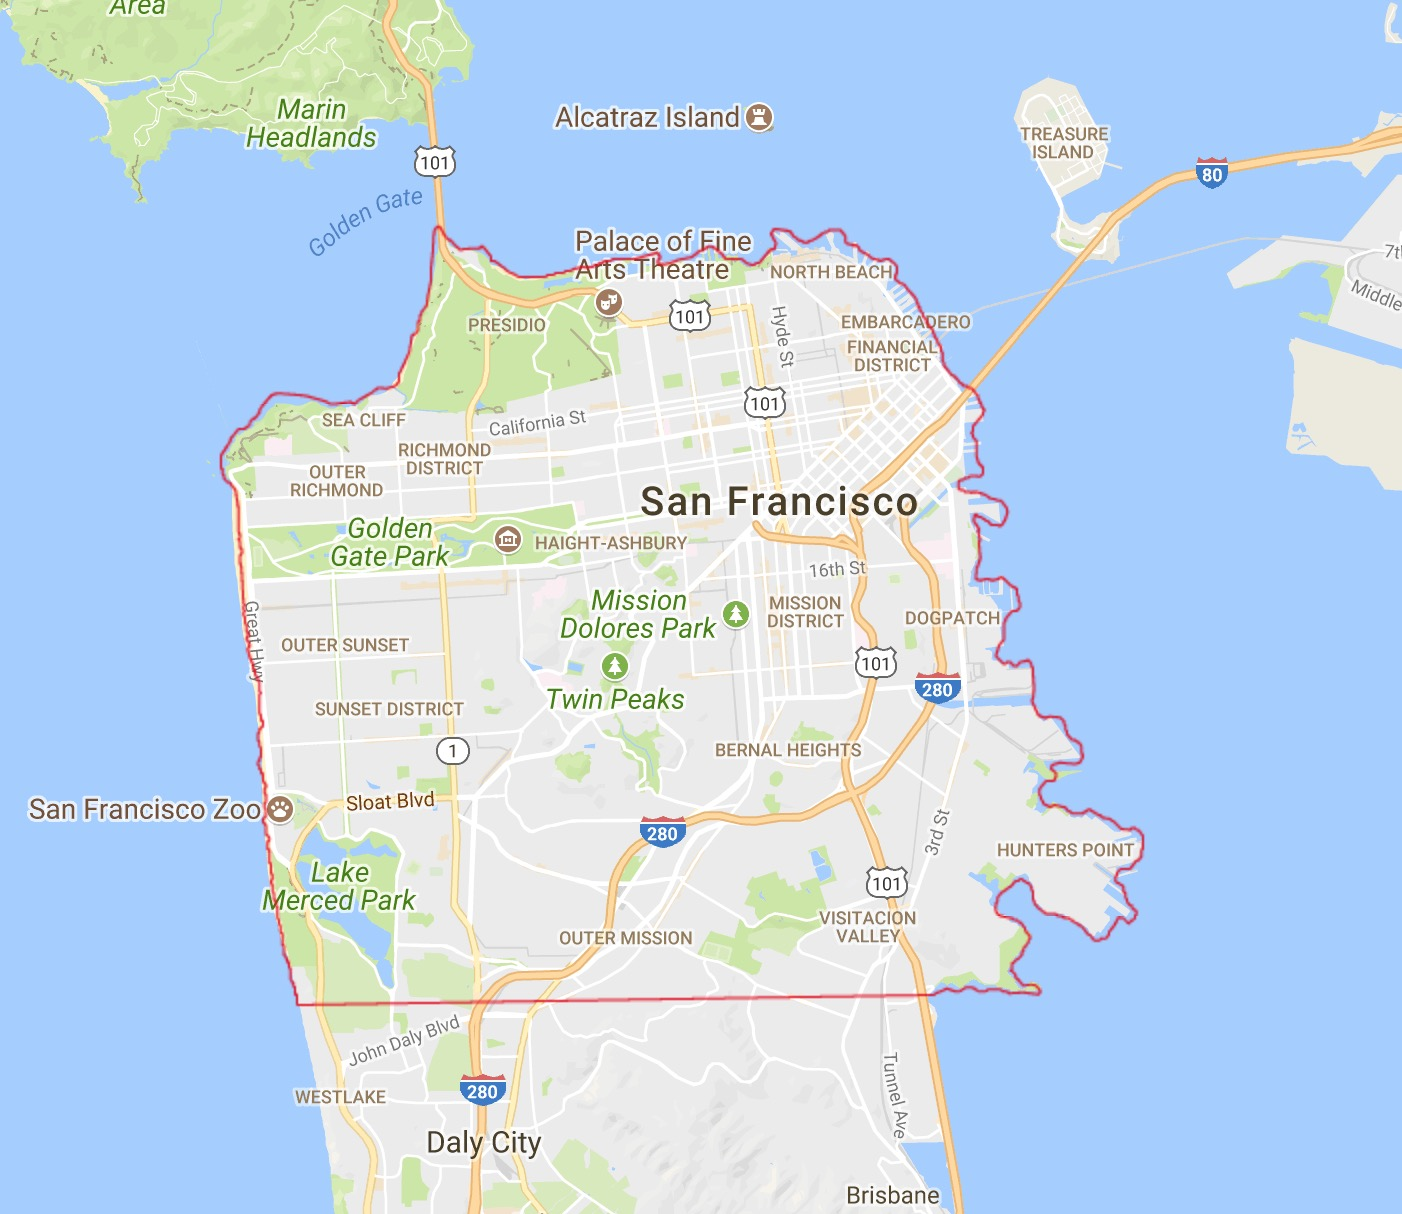
\includegraphics[width=\linewidth]{./images/sanfrancisco.jpg}
            \column{0.4\textwidth}
                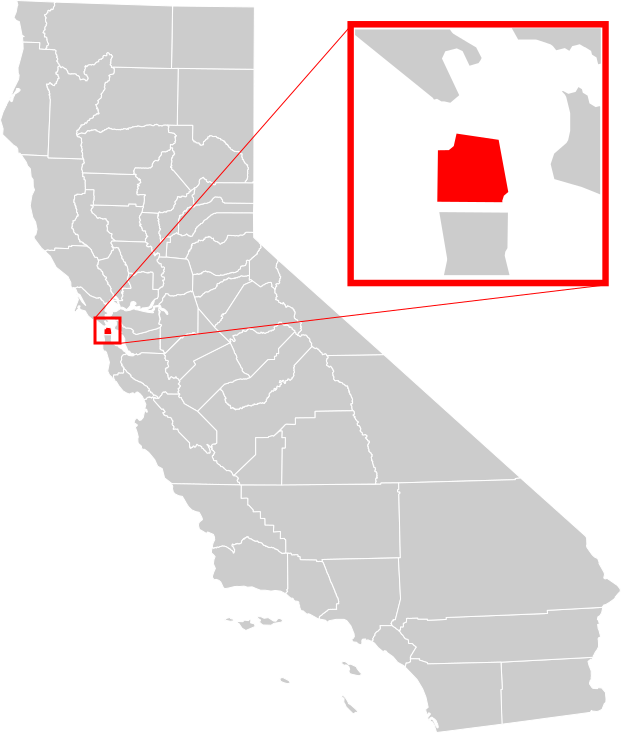
\includegraphics[width=0.7\linewidth]{./images/california-sanfrancisco.png}
                \vskip 1em
                \begin{itemize}
                    \item \scriptsize{Population: 864,816 (2015)}
                    \item \scriptsize{Land Area: 46 $mi^2$}
                \end{itemize}
        \end{columns}
    \end{frame}

    \subsection{Data}                           %subsection 2
    \begin{frame}{Datasets}
        \begin{columns}
        \setbeamercovered{transparent}
            \column{0.5\textwidth}
                \begin{block}{Dataset 1}<1->
                    \begin{itemize}
                        \item
                        \item
                    \end{itemize}
                \end{block}
                \begin{block}{Dataset 2}
                    \begin{itemize}
                        \item
                        \item
                    \end{itemize}
                \end{block}

            \column{0.5\textwidth}
                \begin{block}{Dataset 3}
                    \begin{itemize}
                        \item
                        \item
                    \end{itemize}
                \end{block}
                \begin{block}{Dataset 4}
                    \begin{itemize}
                        \item
                        \item
                    \end{itemize}
                \end{block}
        \setbeamercovered{invisible}
        \end{columns}
    \end{frame}
\end{section}

%------Methodology------%
\begin{section}{Methodology}                     %SECTION 'Methodology'
    \subsection{Design of Framework}             %subsection 1
    \begin{frame}{Design of Framework}
        \begin{itemize}
            \item
            \item
            \item
        \end{itemize}
    \end{frame}

    \subsection{Trainging}                       %subsection 2
    \begin{frame}{Training}
        \begin{itemize}
            \item
            \item
            \item
        \end{itemize}
    \end{frame}

    \subsection{Validation}                      %subsection 3
    \begin{frame}{Validation}
        \begin{itemize}
            \item
            \item
            \item
        \end{itemize}
    \end{frame}
\end{section}

%------References------%
\begin{frame}{References}
    \printbibliography
\end{frame}

%------Thanks------%
\begin{frame}{}
    \begin{center}
    \huge{Thanks!}
    \end{center}
\end{frame}